\documentclass[uplatex,dvipdfmx,a4paper,10pt]{jsarticle}
\usepackage{graphicx}
\usepackage{amsmath}
\usepackage{latexsym}
\usepackage{multirow}
\usepackage{url}
\usepackage[separate-uncertainty]{siunitx}
\usepackage{physics}
\usepackage{enumerate}
\usepackage{bm}
\usepackage{pdfpages}
\usepackage{pxchfon}
\usepackage{tikz}
\usepackage{float}

% tikz setting
\usepackage{tikz}
\usetikzlibrary{automata, intersections, calc, arrows, positioning, arrows.meta}

% \renewcommand{\rmdefault}{pplj}
% \renewcommand{\sfdefault}{phv}

\setlength{\textwidth}{165mm} %165mm-marginparwidth
\setlength{\marginparwidth}{40mm}
\setlength{\textheight}{225mm}
\setlength{\topmargin}{-5mm}
\setlength{\oddsidemargin}{-3.5mm}
% \setlength{\parindent}{0pt}

\def\vector#1{\mbox{\boldmath $#1$}}
\newcommand{\AmSLaTeX}{%
 $\mathcal A$\lower.4ex\hbox{$\!\mathcal M\!$}$\mathcal S$-\LaTeX}
\newcommand{\PS}{{\scshape Post\-Script}}
\def\BibTeX{{\rmfamily B\kern-.05em{\scshape i\kern-.025em b}\kern-.08em
 T\kern-.1667em\lower.7ex\hbox{E}\kern-.125em X}}
\newcommand{\DeLta}{{\mit\Delta}}
\renewcommand{\d}{{\rm d}}
\def\wcaption#1{\caption[]{\parbox[t]{100mm}{#1}}}
\def\rm#1{\mathrm{#1}}
\def\tempC{^\circ \rm{C}}

\makeatletter
\def\section{\@startsection {section}{1}{\z@}{-3.5ex plus -1ex minus -.2ex}{2.3ex plus .2ex}{\Large\bf}}
\def\subsection{\@startsection {subsection}{2}{\z@}{-3.25ex plus -1ex minus -.2ex}{1.5ex plus .2ex}{\normalsize\bf}}
\def\subsubsection{\@startsection {subsubsection}{3}{\z@}{-3.25ex plus -1ex minus -.2ex}{1.5ex plus .2ex}{\small\bf}}
\makeatother

\makeatletter
\def\@seccntformat#1{\@ifundefined{#1@cntformat}%
   {\csname the#1\endcsname\quad}%      default
   {\csname #1@cntformat\endcsname}%    enable individual control
}
\makeatother

\newcommand{\tenexp}[2]{#1\times10^{#2}}


\begin{document}
    % タイトル
    \begin{center}
        {\Large{\bf 形式言語理論 講義13宿題}} \\
        {\bf 2311081 木村慎之介} \\
    \end{center}

    まず右線形文法\(G = (N,\Sigma,P,S)\)に対して、\(G\)が生成する言語\(L(G)\)を受理する\(\lambda\text{-NFA}\ M\)を以下の手順で作る。
    \begin{enumerate}
      \item 以下の方法に基づいて\(G\)を等価な右線形文法\(G^{'} = (N^{'},\ \Sigma,\ P^{'},\ S)\)に変換する。
      \begin{enumerate}
        \item \(P\)の要素について、生成規則が\(A \rightarrow wB(A,\ B \in N,\ w \in \Sigma^{*},\ |w| = n \geq 2,\ w = a_1 \cdots a_n)\)の形で表されるものについては、非終端記号\(A_1,\ \cdots ,\ A_{n-1}\)と次の導出規則\(A \rightarrow a_1A_1,\  A_1 \rightarrow a_2A_2,\ \cdots ,\ A_{n-2} \rightarrow a_{n-1}A_{n-1},\ A_{n-1} \rightarrow a_nB\)を導入して置き換える。
        \item \(P\)の要素について、生成規則が\(A \rightarrow w(A \in N, w \in \Sigma^{*}, |w| = n \geq 2, w = a_1 \cdots a_n)\)の形で表されるものについては、非終端記号\(A_1,\ \cdots ,\ A_{n-1}\)と次の導出規則\(A \rightarrow a_1A_1,\ A_1 \rightarrow a_2A_2,\ \cdots ,\ A_{n-2} \rightarrow a_{n-1}A_{n-1},\ A_{n-1} \rightarrow a_n\)を導入して置き換える。
      \end{enumerate}
      \hspace{1em}このようにすることで任意の\(P^{'}\)に含まれる生成規則は、\(A \rightarrow aB(A,\ B \in N^{'},\ a \in \Sigma \cup \{\lambda\})\)もしくは\(A \rightarrow a(A \in N^{'},\ a \in \Sigma \cup \{\lambda\})\)のいずれかの形で表される。
      \item \(G^{'}\)と同じ言語を受理する\(\lambda \text{-NFA}\ M = (N^{'} \cup \{q_f\},\ \Sigma,\ \delta,\ S,\ \{q_f\})\)の状態遷移関数を以下2パターンに分けて設計する
      \begin{enumerate}
        \item 規則が\(A \rightarrow aB(A,\ B \in N^{'},\ a \in \Sigma \cup \{\lambda\})\)の形で表されるものについて、それに対応する遷移関数を図\ref{picture_state_transition_1}のように定義する。
        
        \begin{figure}[H]
          \centering
          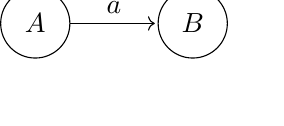
\begin{tikzpicture}[shorten >=1pt, node distance=2cm, on grid, auto]
            \node[state] (A) {\(A\)};
            \node[state] (B) [right=of A]{\(B\)};

            \path[->] (A) edge node {\(a\)} (B);
          \end{tikzpicture}
          \caption{規則\(A \rightarrow aB\)に対応する遷移関数の図}
          \label{picture_state_transition_1}
        \end{figure}

        このとき、同じ文字に対する遷移先は複数個存在して良い。
        \item 規則が\(A \rightarrow a(A \in N^{'},\ a \in \Sigma \cup \{\lambda\})\)の形で表されるものについて、それに対応する遷移関数を図\ref{picture_state_transition_2}のように定義する。
        
        \begin{figure}[H]
          \centering
          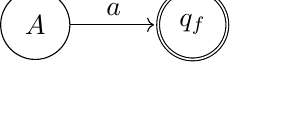
\begin{tikzpicture}[shorten >=1pt, node distance=2cm, on grid, auto]
            \node[state] (A) {\(A\)};
            \node[state, accepting] [right=of A](q_f) {\(q_f\)};

            \path[->] (A) edge node {\(a\)} (q_f);
          \end{tikzpicture}
          \caption{規則\(A \rightarrow a\)に対応する遷移関数の図}
          \label{picture_state_transition_2}
        \end{figure}

      \end{enumerate}
    \end{enumerate}
    \hspace{1em}最後に作成した\(M\)の受理する言語\(L(M)\)が\(L(G)\)と等しいことを\(L(A) = L(G^{'})\)であることから証明する。\\
    \hspace{1em}\(w \in L(G^{'})\)を仮定する。
    この\(w\)は\(G^{'}\)によって\(S \Rightarrow_G a_1A_1 \Rightarrow_G \cdots \Rightarrow_G a_1 \cdots a_{n-1}A_{n-1} \Rightarrow_G a_1 \cdots a_n\)と生成されるとする。
    この時、\(w\)を\(M\)に入力すると\(S \xrightarrow{a_1} A_1 \xrightarrow{a_2} \cdots \xrightarrow{a_n} q_f\)と状態が遷移して受理される。
    よって\(w \in L(M)\)である。 \\
    \hspace{1em}逆に\(w = a_1 \cdots a_n \in L(M)\)の時、\(M\)は\(w\)を\(S \xrightarrow{a_1} A_1 \xrightarrow{a_2} \cdots \xrightarrow{a_n} q_f\)と受理される。
    このとき、\(M\)の状態遷移関数と\(G^{'}\)の生成規則の対応関係から\(G^{'}\)が\(w\)を\(S \Rightarrow_G a_1A_1 \Rightarrow_G \cdots \Rightarrow_G a_1 \cdots a_{n-1}A_{n-1} \Rightarrow_G a_1 \cdots a_n\)と生成することがわかる。
    よって\(w \in L(G^{'})\)となる。 \\
    \hspace{1em}以上より\(L(M) = L(G^{'})\)が証明され、\(G^{'}\)と\(G\)が等価であることから\(L(M) = L(G)\)となり、Gが正則であると証明された。

    %%%%%%%%%%%%%%%%%%%%%%%%%%%%%%%%%%%%%%%%%%%%%%%%%%%%%%%%%%%%%%%%%%%%%%
    \appendix
    \setcounter{figure}{0}
    \setcounter{table}{0}
    \numberwithin{equation}{section}
    \renewcommand{\thetable}{\Alph{section}\arabic{table}}
    \renewcommand{\thefigure}{\Alph{section}\arabic{figure}}
    %\def\thesection{付録\Alph{section}}
    \makeatletter 
    \newcommand{\section@cntformat}{付録 \thesection:\ }
    \makeatother
    %%%%%%%%%%%%%%%%%%%%%%%%%%%%%%%%%%%%%%%%%%%%%%%%%%%%%%%%%%%%%%%%%%%%%%
    
    
\end{document}